% Options for packages loaded elsewhere
\PassOptionsToPackage{unicode}{hyperref}
\PassOptionsToPackage{hyphens}{url}
%
\documentclass[
]{article}
\usepackage{amsmath,amssymb}
\usepackage{lmodern}
\usepackage{iftex}
\ifPDFTeX
  \usepackage[T1]{fontenc}
  \usepackage[utf8]{inputenc}
  \usepackage{textcomp} % provide euro and other symbols
\else % if luatex or xetex
  \usepackage{unicode-math}
  \defaultfontfeatures{Scale=MatchLowercase}
  \defaultfontfeatures[\rmfamily]{Ligatures=TeX,Scale=1}
\fi
% Use upquote if available, for straight quotes in verbatim environments
\IfFileExists{upquote.sty}{\usepackage{upquote}}{}
\IfFileExists{microtype.sty}{% use microtype if available
  \usepackage[]{microtype}
  \UseMicrotypeSet[protrusion]{basicmath} % disable protrusion for tt fonts
}{}
\makeatletter
\@ifundefined{KOMAClassName}{% if non-KOMA class
  \IfFileExists{parskip.sty}{%
    \usepackage{parskip}
  }{% else
    \setlength{\parindent}{0pt}
    \setlength{\parskip}{6pt plus 2pt minus 1pt}}
}{% if KOMA class
  \KOMAoptions{parskip=half}}
\makeatother
\usepackage{xcolor}
\usepackage[margin=1in]{geometry}
\usepackage{color}
\usepackage{fancyvrb}
\newcommand{\VerbBar}{|}
\newcommand{\VERB}{\Verb[commandchars=\\\{\}]}
\DefineVerbatimEnvironment{Highlighting}{Verbatim}{commandchars=\\\{\}}
% Add ',fontsize=\small' for more characters per line
\usepackage{framed}
\definecolor{shadecolor}{RGB}{248,248,248}
\newenvironment{Shaded}{\begin{snugshade}}{\end{snugshade}}
\newcommand{\AlertTok}[1]{\textcolor[rgb]{0.94,0.16,0.16}{#1}}
\newcommand{\AnnotationTok}[1]{\textcolor[rgb]{0.56,0.35,0.01}{\textbf{\textit{#1}}}}
\newcommand{\AttributeTok}[1]{\textcolor[rgb]{0.77,0.63,0.00}{#1}}
\newcommand{\BaseNTok}[1]{\textcolor[rgb]{0.00,0.00,0.81}{#1}}
\newcommand{\BuiltInTok}[1]{#1}
\newcommand{\CharTok}[1]{\textcolor[rgb]{0.31,0.60,0.02}{#1}}
\newcommand{\CommentTok}[1]{\textcolor[rgb]{0.56,0.35,0.01}{\textit{#1}}}
\newcommand{\CommentVarTok}[1]{\textcolor[rgb]{0.56,0.35,0.01}{\textbf{\textit{#1}}}}
\newcommand{\ConstantTok}[1]{\textcolor[rgb]{0.00,0.00,0.00}{#1}}
\newcommand{\ControlFlowTok}[1]{\textcolor[rgb]{0.13,0.29,0.53}{\textbf{#1}}}
\newcommand{\DataTypeTok}[1]{\textcolor[rgb]{0.13,0.29,0.53}{#1}}
\newcommand{\DecValTok}[1]{\textcolor[rgb]{0.00,0.00,0.81}{#1}}
\newcommand{\DocumentationTok}[1]{\textcolor[rgb]{0.56,0.35,0.01}{\textbf{\textit{#1}}}}
\newcommand{\ErrorTok}[1]{\textcolor[rgb]{0.64,0.00,0.00}{\textbf{#1}}}
\newcommand{\ExtensionTok}[1]{#1}
\newcommand{\FloatTok}[1]{\textcolor[rgb]{0.00,0.00,0.81}{#1}}
\newcommand{\FunctionTok}[1]{\textcolor[rgb]{0.00,0.00,0.00}{#1}}
\newcommand{\ImportTok}[1]{#1}
\newcommand{\InformationTok}[1]{\textcolor[rgb]{0.56,0.35,0.01}{\textbf{\textit{#1}}}}
\newcommand{\KeywordTok}[1]{\textcolor[rgb]{0.13,0.29,0.53}{\textbf{#1}}}
\newcommand{\NormalTok}[1]{#1}
\newcommand{\OperatorTok}[1]{\textcolor[rgb]{0.81,0.36,0.00}{\textbf{#1}}}
\newcommand{\OtherTok}[1]{\textcolor[rgb]{0.56,0.35,0.01}{#1}}
\newcommand{\PreprocessorTok}[1]{\textcolor[rgb]{0.56,0.35,0.01}{\textit{#1}}}
\newcommand{\RegionMarkerTok}[1]{#1}
\newcommand{\SpecialCharTok}[1]{\textcolor[rgb]{0.00,0.00,0.00}{#1}}
\newcommand{\SpecialStringTok}[1]{\textcolor[rgb]{0.31,0.60,0.02}{#1}}
\newcommand{\StringTok}[1]{\textcolor[rgb]{0.31,0.60,0.02}{#1}}
\newcommand{\VariableTok}[1]{\textcolor[rgb]{0.00,0.00,0.00}{#1}}
\newcommand{\VerbatimStringTok}[1]{\textcolor[rgb]{0.31,0.60,0.02}{#1}}
\newcommand{\WarningTok}[1]{\textcolor[rgb]{0.56,0.35,0.01}{\textbf{\textit{#1}}}}
\usepackage{graphicx}
\makeatletter
\def\maxwidth{\ifdim\Gin@nat@width>\linewidth\linewidth\else\Gin@nat@width\fi}
\def\maxheight{\ifdim\Gin@nat@height>\textheight\textheight\else\Gin@nat@height\fi}
\makeatother
% Scale images if necessary, so that they will not overflow the page
% margins by default, and it is still possible to overwrite the defaults
% using explicit options in \includegraphics[width, height, ...]{}
\setkeys{Gin}{width=\maxwidth,height=\maxheight,keepaspectratio}
% Set default figure placement to htbp
\makeatletter
\def\fps@figure{htbp}
\makeatother
\setlength{\emergencystretch}{3em} % prevent overfull lines
\providecommand{\tightlist}{%
  \setlength{\itemsep}{0pt}\setlength{\parskip}{0pt}}
\setcounter{secnumdepth}{-\maxdimen} % remove section numbering
\ifLuaTeX
  \usepackage{selnolig}  % disable illegal ligatures
\fi
\IfFileExists{bookmark.sty}{\usepackage{bookmark}}{\usepackage{hyperref}}
\IfFileExists{xurl.sty}{\usepackage{xurl}}{} % add URL line breaks if available
\urlstyle{same} % disable monospaced font for URLs
\hypersetup{
  hidelinks,
  pdfcreator={LaTeX via pandoc}}

\author{}
\date{\vspace{-2.5em}}

\begin{document}

\hypertarget{packages-libraries}{%
\subsubsection{Packages \& Libraries}\label{packages-libraries}}

\begin{Shaded}
\begin{Highlighting}[]
\FunctionTok{library}\NormalTok{(corrplot)}
\end{Highlighting}
\end{Shaded}

\begin{verbatim}
## corrplot 0.92 loaded
\end{verbatim}

\begin{Shaded}
\begin{Highlighting}[]
\FunctionTok{library}\NormalTok{(ggplot2)}
\FunctionTok{library}\NormalTok{(caret)}
\end{Highlighting}
\end{Shaded}

\begin{verbatim}
## Loading required package: lattice
\end{verbatim}

\begin{Shaded}
\begin{Highlighting}[]
\FunctionTok{library}\NormalTok{(mlbench)}
\FunctionTok{library}\NormalTok{(ROCR)}
\FunctionTok{library}\NormalTok{(party)}
\end{Highlighting}
\end{Shaded}

\begin{verbatim}
## Loading required package: grid
\end{verbatim}

\begin{verbatim}
## Loading required package: mvtnorm
\end{verbatim}

\begin{verbatim}
## Loading required package: modeltools
\end{verbatim}

\begin{verbatim}
## Loading required package: stats4
\end{verbatim}

\begin{verbatim}
## Loading required package: strucchange
\end{verbatim}

\begin{verbatim}
## Loading required package: zoo
\end{verbatim}

\begin{verbatim}
## 
## Attaching package: 'zoo'
\end{verbatim}

\begin{verbatim}
## The following objects are masked from 'package:base':
## 
##     as.Date, as.Date.numeric
\end{verbatim}

\begin{verbatim}
## Loading required package: sandwich
\end{verbatim}

\begin{Shaded}
\begin{Highlighting}[]
\FunctionTok{library}\NormalTok{(rpart)}
\end{Highlighting}
\end{Shaded}

\hypertarget{preprocessing}{%
\subsubsection{Preprocessing}\label{preprocessing}}

\begin{Shaded}
\begin{Highlighting}[]
\NormalTok{data }\OtherTok{\textless{}{-}} \FunctionTok{read.csv}\NormalTok{(}\StringTok{"bank{-}additional{-}full.csv"}\NormalTok{,}\AttributeTok{sep=}\StringTok{";"}\NormalTok{)}
\FunctionTok{head}\NormalTok{(data)}
\end{Highlighting}
\end{Shaded}

\begin{verbatim}
##   age       job marital   education default housing loan   contact month
## 1  56 housemaid married    basic.4y      no      no   no telephone   may
## 2  57  services married high.school unknown      no   no telephone   may
## 3  37  services married high.school      no     yes   no telephone   may
## 4  40    admin. married    basic.6y      no      no   no telephone   may
## 5  56  services married high.school      no      no  yes telephone   may
## 6  45  services married    basic.9y unknown      no   no telephone   may
##   day_of_week duration campaign pdays previous    poutcome emp.var.rate
## 1         mon      261        1   999        0 nonexistent          1.1
## 2         mon      149        1   999        0 nonexistent          1.1
## 3         mon      226        1   999        0 nonexistent          1.1
## 4         mon      151        1   999        0 nonexistent          1.1
## 5         mon      307        1   999        0 nonexistent          1.1
## 6         mon      198        1   999        0 nonexistent          1.1
##   cons.price.idx cons.conf.idx euribor3m nr.employed  y
## 1         93.994         -36.4     4.857        5191 no
## 2         93.994         -36.4     4.857        5191 no
## 3         93.994         -36.4     4.857        5191 no
## 4         93.994         -36.4     4.857        5191 no
## 5         93.994         -36.4     4.857        5191 no
## 6         93.994         -36.4     4.857        5191 no
\end{verbatim}

showing row count

\begin{Shaded}
\begin{Highlighting}[]
\FunctionTok{cat}\NormalTok{(}\StringTok{"Original row count is"}\NormalTok{,}\FunctionTok{nrow}\NormalTok{(data))}
\end{Highlighting}
\end{Shaded}

\begin{verbatim}
## Original row count is 41188
\end{verbatim}

dropping `duration',`pdays',`default'

\begin{Shaded}
\begin{Highlighting}[]
\NormalTok{data }\OtherTok{\textless{}{-}} \FunctionTok{subset}\NormalTok{(data, }\AttributeTok{select =} \SpecialCharTok{{-}}\FunctionTok{c}\NormalTok{(duration, pdays, default))}
\FunctionTok{colnames}\NormalTok{(data)}
\end{Highlighting}
\end{Shaded}

\begin{verbatim}
##  [1] "age"            "job"            "marital"        "education"     
##  [5] "housing"        "loan"           "contact"        "month"         
##  [9] "day_of_week"    "campaign"       "previous"       "poutcome"      
## [13] "emp.var.rate"   "cons.price.idx" "cons.conf.idx"  "euribor3m"     
## [17] "nr.employed"    "y"
\end{verbatim}

find the columns that have ``unknown'' as a value

\begin{Shaded}
\begin{Highlighting}[]
\NormalTok{has\_unknown }\OtherTok{\textless{}{-}} \ControlFlowTok{function}\NormalTok{(df, col) \{}
\NormalTok{  (}\FunctionTok{sum}\NormalTok{(df[,col]}\SpecialCharTok{==}\StringTok{"unknown"}\NormalTok{)}\SpecialCharTok{\textgreater{}}\DecValTok{0}\NormalTok{)}
\NormalTok{\}}
\NormalTok{where\_is\_unknown }\OtherTok{\textless{}{-}} \ControlFlowTok{function}\NormalTok{(df) \{}
\NormalTok{  c }\OtherTok{\textless{}{-}} \DecValTok{0}
  \ControlFlowTok{for}\NormalTok{(col }\ControlFlowTok{in} \FunctionTok{colnames}\NormalTok{(df)) \{}
    \ControlFlowTok{if}\NormalTok{ (}\FunctionTok{has\_unknown}\NormalTok{(df,col)) \{}
      \FunctionTok{cat}\NormalTok{(col)}
\NormalTok{      c }\OtherTok{\textless{}{-}}\NormalTok{ c }\SpecialCharTok{+} \DecValTok{1}
\NormalTok{    \}}
\NormalTok{  \}}
  \ControlFlowTok{if}\NormalTok{(c }\SpecialCharTok{==} \DecValTok{0}\NormalTok{) \{}
    \FunctionTok{print}\NormalTok{(}\FunctionTok{paste}\NormalTok{(}\StringTok{"There are no unknown values in the dataframe"}\NormalTok{))}
\NormalTok{  \}}
\NormalTok{\}}
\FunctionTok{print}\NormalTok{(}\FunctionTok{paste}\NormalTok{(}\StringTok{"These columns have unknown values"}\NormalTok{))}
\end{Highlighting}
\end{Shaded}

\begin{verbatim}
## [1] "These columns have unknown values"
\end{verbatim}

\begin{Shaded}
\begin{Highlighting}[]
\FunctionTok{where\_is\_unknown}\NormalTok{(data)}
\end{Highlighting}
\end{Shaded}

\begin{verbatim}
## jobmaritaleducationhousingloan
\end{verbatim}

replace those ``unknown'' values with a sample of the other values in
those columns

\begin{Shaded}
\begin{Highlighting}[]
\NormalTok{replace\_unknowns }\OtherTok{\textless{}{-}} \ControlFlowTok{function}\NormalTok{(df) \{}
  \ControlFlowTok{for}\NormalTok{(col }\ControlFlowTok{in} \FunctionTok{colnames}\NormalTok{(df)) \{}
    \ControlFlowTok{if}\NormalTok{(}\FunctionTok{has\_unknown}\NormalTok{(df,col)) \{}
\NormalTok{      n\_unk }\OtherTok{\textless{}{-}} \FunctionTok{sum}\NormalTok{(df[,col]}\SpecialCharTok{==}\StringTok{"unknown"}\NormalTok{)}
\NormalTok{      idx }\OtherTok{\textless{}{-}} \FunctionTok{which}\NormalTok{(df[,col]}\SpecialCharTok{==}\StringTok{"unknown"}\NormalTok{)}
\NormalTok{      df[idx,col] }\OtherTok{\textless{}{-}} \FunctionTok{sample}\NormalTok{(col[}\SpecialCharTok{!}\NormalTok{col}\SpecialCharTok{==}\StringTok{"unknown"}\NormalTok{],n\_unk,}\AttributeTok{replace=}\ConstantTok{TRUE}\NormalTok{)}
\NormalTok{    \}}
\NormalTok{  \}}
\NormalTok{  df}
\NormalTok{\}}
\NormalTok{data }\OtherTok{\textless{}{-}} \FunctionTok{replace\_unknowns}\NormalTok{(data)}
\FunctionTok{head}\NormalTok{(data)}
\end{Highlighting}
\end{Shaded}

\begin{verbatim}
##   age       job marital   education housing loan   contact month day_of_week
## 1  56 housemaid married    basic.4y      no   no telephone   may         mon
## 2  57  services married high.school      no   no telephone   may         mon
## 3  37  services married high.school     yes   no telephone   may         mon
## 4  40    admin. married    basic.6y      no   no telephone   may         mon
## 5  56  services married high.school      no  yes telephone   may         mon
## 6  45  services married    basic.9y      no   no telephone   may         mon
##   campaign previous    poutcome emp.var.rate cons.price.idx cons.conf.idx
## 1        1        0 nonexistent          1.1         93.994         -36.4
## 2        1        0 nonexistent          1.1         93.994         -36.4
## 3        1        0 nonexistent          1.1         93.994         -36.4
## 4        1        0 nonexistent          1.1         93.994         -36.4
## 5        1        0 nonexistent          1.1         93.994         -36.4
## 6        1        0 nonexistent          1.1         93.994         -36.4
##   euribor3m nr.employed  y
## 1     4.857        5191 no
## 2     4.857        5191 no
## 3     4.857        5191 no
## 4     4.857        5191 no
## 5     4.857        5191 no
## 6     4.857        5191 no
\end{verbatim}

just to make sure those values were actually replaced and now there's no
more unknowns

\begin{Shaded}
\begin{Highlighting}[]
\FunctionTok{cat}\NormalTok{(}\StringTok{"\# of unknowns:"}\NormalTok{, }\FunctionTok{sum}\NormalTok{(data}\SpecialCharTok{==}\StringTok{"unknown"}\NormalTok{))}
\end{Highlighting}
\end{Shaded}

\begin{verbatim}
## # of unknowns: 0
\end{verbatim}

show the categorical columns

\begin{Shaded}
\begin{Highlighting}[]
\NormalTok{cats }\OtherTok{\textless{}{-}} \FunctionTok{names}\NormalTok{(data)[}\FunctionTok{sapply}\NormalTok{(data,is.character)]}
\NormalTok{cats}
\end{Highlighting}
\end{Shaded}

\begin{verbatim}
##  [1] "job"         "marital"     "education"   "housing"     "loan"       
##  [6] "contact"     "month"       "day_of_week" "poutcome"    "y"
\end{verbatim}

encode all of the categorical values into numericals

\begin{Shaded}
\begin{Highlighting}[]
\NormalTok{encode }\OtherTok{\textless{}{-}} \ControlFlowTok{function}\NormalTok{(df,col) \{}
  \FunctionTok{as.numeric}\NormalTok{(}\FunctionTok{factor}\NormalTok{(df[,col]))}\SpecialCharTok{{-}}\DecValTok{1}
\NormalTok{\}}
\ControlFlowTok{for}\NormalTok{(cat }\ControlFlowTok{in}\NormalTok{ cats) \{}
\NormalTok{  data[,cat] }\OtherTok{\textless{}{-}} \FunctionTok{encode}\NormalTok{(data,cat)}
\NormalTok{\}}
\FunctionTok{head}\NormalTok{(data)}
\end{Highlighting}
\end{Shaded}

\begin{verbatim}
##   age job marital education housing loan contact month day_of_week campaign
## 1  56   3       2         0       1    1       1     6           1        1
## 2  57   8       2         4       1    1       1     6           1        1
## 3  37   8       2         4       2    1       1     6           1        1
## 4  40   0       2         1       1    1       1     6           1        1
## 5  56   8       2         4       1    2       1     6           1        1
## 6  45   8       2         2       1    1       1     6           1        1
##   previous poutcome emp.var.rate cons.price.idx cons.conf.idx euribor3m
## 1        0        1          1.1         93.994         -36.4     4.857
## 2        0        1          1.1         93.994         -36.4     4.857
## 3        0        1          1.1         93.994         -36.4     4.857
## 4        0        1          1.1         93.994         -36.4     4.857
## 5        0        1          1.1         93.994         -36.4     4.857
## 6        0        1          1.1         93.994         -36.4     4.857
##   nr.employed y
## 1        5191 0
## 2        5191 0
## 3        5191 0
## 4        5191 0
## 5        5191 0
## 6        5191 0
\end{verbatim}

count plot for target to check for imbalance

\begin{Shaded}
\begin{Highlighting}[]
\NormalTok{plt }\OtherTok{\textless{}{-}} \FunctionTok{ggplot}\NormalTok{(data, }\FunctionTok{aes}\NormalTok{(}\AttributeTok{x =}\NormalTok{ y)) }\SpecialCharTok{+} \FunctionTok{geom\_bar}\NormalTok{(}\AttributeTok{size=}\DecValTok{6}\NormalTok{) }
\NormalTok{plt }\SpecialCharTok{+} \FunctionTok{ggtitle}\NormalTok{(}\StringTok{"}\SpecialCharTok{\textbackslash{}t\textbackslash{}t\textbackslash{}t\textbackslash{}t}\StringTok{Class Imbalance in y"}\NormalTok{)}
\end{Highlighting}
\end{Shaded}

\begin{verbatim}
## Warning in grid.Call(C_textBounds, as.graphicsAnnot(x$label), x$x, x$y, : font
## width unknown for character 0x9

## Warning in grid.Call(C_textBounds, as.graphicsAnnot(x$label), x$x, x$y, : font
## width unknown for character 0x9

## Warning in grid.Call(C_textBounds, as.graphicsAnnot(x$label), x$x, x$y, : font
## width unknown for character 0x9

## Warning in grid.Call(C_textBounds, as.graphicsAnnot(x$label), x$x, x$y, : font
## width unknown for character 0x9

## Warning in grid.Call(C_textBounds, as.graphicsAnnot(x$label), x$x, x$y, : font
## width unknown for character 0x9

## Warning in grid.Call(C_textBounds, as.graphicsAnnot(x$label), x$x, x$y, : font
## width unknown for character 0x9

## Warning in grid.Call(C_textBounds, as.graphicsAnnot(x$label), x$x, x$y, : font
## width unknown for character 0x9

## Warning in grid.Call(C_textBounds, as.graphicsAnnot(x$label), x$x, x$y, : font
## width unknown for character 0x9

## Warning in grid.Call(C_textBounds, as.graphicsAnnot(x$label), x$x, x$y, : font
## width unknown for character 0x9

## Warning in grid.Call(C_textBounds, as.graphicsAnnot(x$label), x$x, x$y, : font
## width unknown for character 0x9

## Warning in grid.Call(C_textBounds, as.graphicsAnnot(x$label), x$x, x$y, : font
## width unknown for character 0x9

## Warning in grid.Call(C_textBounds, as.graphicsAnnot(x$label), x$x, x$y, : font
## width unknown for character 0x9

## Warning in grid.Call(C_textBounds, as.graphicsAnnot(x$label), x$x, x$y, : font
## width unknown for character 0x9

## Warning in grid.Call(C_textBounds, as.graphicsAnnot(x$label), x$x, x$y, : font
## width unknown for character 0x9

## Warning in grid.Call(C_textBounds, as.graphicsAnnot(x$label), x$x, x$y, : font
## width unknown for character 0x9

## Warning in grid.Call(C_textBounds, as.graphicsAnnot(x$label), x$x, x$y, : font
## width unknown for character 0x9

## Warning in grid.Call(C_textBounds, as.graphicsAnnot(x$label), x$x, x$y, : font
## width unknown for character 0x9

## Warning in grid.Call(C_textBounds, as.graphicsAnnot(x$label), x$x, x$y, : font
## width unknown for character 0x9

## Warning in grid.Call(C_textBounds, as.graphicsAnnot(x$label), x$x, x$y, : font
## width unknown for character 0x9

## Warning in grid.Call(C_textBounds, as.graphicsAnnot(x$label), x$x, x$y, : font
## width unknown for character 0x9

## Warning in grid.Call(C_textBounds, as.graphicsAnnot(x$label), x$x, x$y, : font
## width unknown for character 0x9

## Warning in grid.Call(C_textBounds, as.graphicsAnnot(x$label), x$x, x$y, : font
## width unknown for character 0x9

## Warning in grid.Call(C_textBounds, as.graphicsAnnot(x$label), x$x, x$y, : font
## width unknown for character 0x9

## Warning in grid.Call(C_textBounds, as.graphicsAnnot(x$label), x$x, x$y, : font
## width unknown for character 0x9

## Warning in grid.Call(C_textBounds, as.graphicsAnnot(x$label), x$x, x$y, : font
## width unknown for character 0x9

## Warning in grid.Call(C_textBounds, as.graphicsAnnot(x$label), x$x, x$y, : font
## width unknown for character 0x9

## Warning in grid.Call(C_textBounds, as.graphicsAnnot(x$label), x$x, x$y, : font
## width unknown for character 0x9

## Warning in grid.Call(C_textBounds, as.graphicsAnnot(x$label), x$x, x$y, : font
## width unknown for character 0x9
\end{verbatim}

\begin{verbatim}
## Warning in grid.Call.graphics(C_text, as.graphicsAnnot(x$label), x$x, x$y, :
## font width unknown for character 0x9

## Warning in grid.Call.graphics(C_text, as.graphicsAnnot(x$label), x$x, x$y, :
## font width unknown for character 0x9

## Warning in grid.Call.graphics(C_text, as.graphicsAnnot(x$label), x$x, x$y, :
## font width unknown for character 0x9

## Warning in grid.Call.graphics(C_text, as.graphicsAnnot(x$label), x$x, x$y, :
## font width unknown for character 0x9
\end{verbatim}

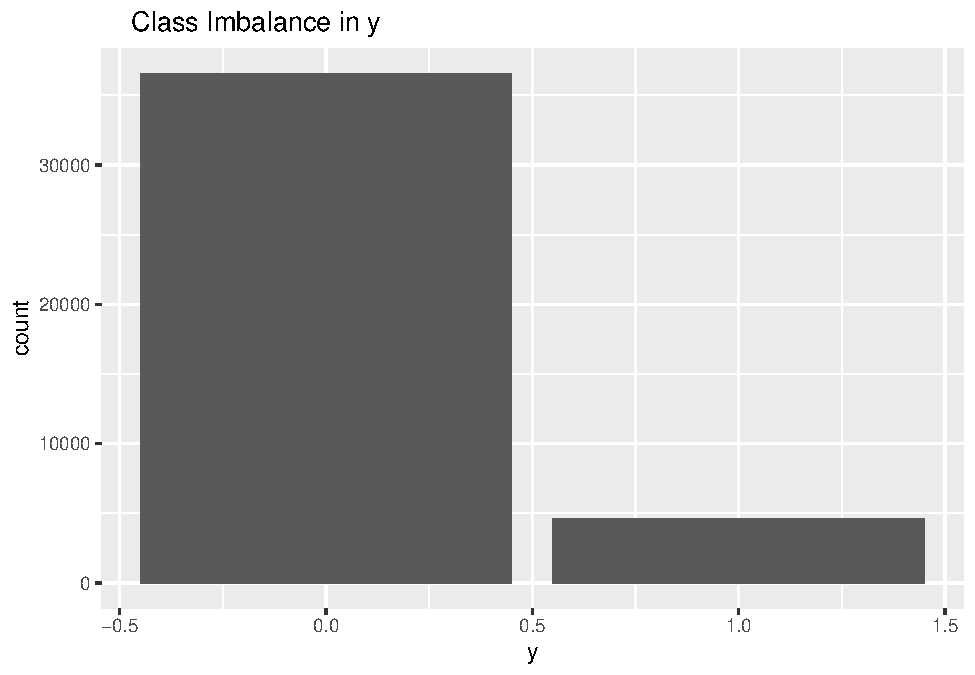
\includegraphics{part1_files/figure-latex/unnamed-chunk-10-1.pdf}

Fixing the class imbalance by oversampling \& resetting dataframe

\begin{Shaded}
\begin{Highlighting}[]
\NormalTok{data}\SpecialCharTok{$}\NormalTok{y }\OtherTok{\textless{}{-}} \FunctionTok{factor}\NormalTok{(data}\SpecialCharTok{$}\NormalTok{y)}
\NormalTok{data }\OtherTok{\textless{}{-}} \FunctionTok{upSample}\NormalTok{(}\AttributeTok{x=}\NormalTok{data[,}\SpecialCharTok{{-}}\FunctionTok{ncol}\NormalTok{(data)],}\AttributeTok{y=}\NormalTok{data}\SpecialCharTok{$}\NormalTok{y)}
\FunctionTok{names}\NormalTok{(data)[}\FunctionTok{names}\NormalTok{(data)}\SpecialCharTok{==}\StringTok{\textquotesingle{}Class\textquotesingle{}}\NormalTok{] }\OtherTok{\textless{}{-}} \StringTok{\textquotesingle{}y\textquotesingle{}}
\end{Highlighting}
\end{Shaded}

count plot for target to ensure classes have been balanced

\begin{Shaded}
\begin{Highlighting}[]
\NormalTok{plt }\OtherTok{\textless{}{-}} \FunctionTok{ggplot}\NormalTok{(data, }\FunctionTok{aes}\NormalTok{(}\AttributeTok{x =}\NormalTok{ y)) }\SpecialCharTok{+} \FunctionTok{geom\_bar}\NormalTok{(}\AttributeTok{size=}\DecValTok{6}\NormalTok{) }
\NormalTok{plt }\SpecialCharTok{+} \FunctionTok{ggtitle}\NormalTok{(}\StringTok{"}\SpecialCharTok{\textbackslash{}t\textbackslash{}t\textbackslash{}t\textbackslash{}t}\StringTok{Class Balance in y"}\NormalTok{)}
\end{Highlighting}
\end{Shaded}

\begin{verbatim}
## Warning in grid.Call(C_textBounds, as.graphicsAnnot(x$label), x$x, x$y, : font
## width unknown for character 0x9

## Warning in grid.Call(C_textBounds, as.graphicsAnnot(x$label), x$x, x$y, : font
## width unknown for character 0x9

## Warning in grid.Call(C_textBounds, as.graphicsAnnot(x$label), x$x, x$y, : font
## width unknown for character 0x9

## Warning in grid.Call(C_textBounds, as.graphicsAnnot(x$label), x$x, x$y, : font
## width unknown for character 0x9

## Warning in grid.Call(C_textBounds, as.graphicsAnnot(x$label), x$x, x$y, : font
## width unknown for character 0x9

## Warning in grid.Call(C_textBounds, as.graphicsAnnot(x$label), x$x, x$y, : font
## width unknown for character 0x9

## Warning in grid.Call(C_textBounds, as.graphicsAnnot(x$label), x$x, x$y, : font
## width unknown for character 0x9

## Warning in grid.Call(C_textBounds, as.graphicsAnnot(x$label), x$x, x$y, : font
## width unknown for character 0x9

## Warning in grid.Call(C_textBounds, as.graphicsAnnot(x$label), x$x, x$y, : font
## width unknown for character 0x9

## Warning in grid.Call(C_textBounds, as.graphicsAnnot(x$label), x$x, x$y, : font
## width unknown for character 0x9

## Warning in grid.Call(C_textBounds, as.graphicsAnnot(x$label), x$x, x$y, : font
## width unknown for character 0x9

## Warning in grid.Call(C_textBounds, as.graphicsAnnot(x$label), x$x, x$y, : font
## width unknown for character 0x9

## Warning in grid.Call(C_textBounds, as.graphicsAnnot(x$label), x$x, x$y, : font
## width unknown for character 0x9

## Warning in grid.Call(C_textBounds, as.graphicsAnnot(x$label), x$x, x$y, : font
## width unknown for character 0x9

## Warning in grid.Call(C_textBounds, as.graphicsAnnot(x$label), x$x, x$y, : font
## width unknown for character 0x9

## Warning in grid.Call(C_textBounds, as.graphicsAnnot(x$label), x$x, x$y, : font
## width unknown for character 0x9

## Warning in grid.Call(C_textBounds, as.graphicsAnnot(x$label), x$x, x$y, : font
## width unknown for character 0x9

## Warning in grid.Call(C_textBounds, as.graphicsAnnot(x$label), x$x, x$y, : font
## width unknown for character 0x9

## Warning in grid.Call(C_textBounds, as.graphicsAnnot(x$label), x$x, x$y, : font
## width unknown for character 0x9

## Warning in grid.Call(C_textBounds, as.graphicsAnnot(x$label), x$x, x$y, : font
## width unknown for character 0x9

## Warning in grid.Call(C_textBounds, as.graphicsAnnot(x$label), x$x, x$y, : font
## width unknown for character 0x9

## Warning in grid.Call(C_textBounds, as.graphicsAnnot(x$label), x$x, x$y, : font
## width unknown for character 0x9

## Warning in grid.Call(C_textBounds, as.graphicsAnnot(x$label), x$x, x$y, : font
## width unknown for character 0x9

## Warning in grid.Call(C_textBounds, as.graphicsAnnot(x$label), x$x, x$y, : font
## width unknown for character 0x9

## Warning in grid.Call(C_textBounds, as.graphicsAnnot(x$label), x$x, x$y, : font
## width unknown for character 0x9

## Warning in grid.Call(C_textBounds, as.graphicsAnnot(x$label), x$x, x$y, : font
## width unknown for character 0x9

## Warning in grid.Call(C_textBounds, as.graphicsAnnot(x$label), x$x, x$y, : font
## width unknown for character 0x9

## Warning in grid.Call(C_textBounds, as.graphicsAnnot(x$label), x$x, x$y, : font
## width unknown for character 0x9
\end{verbatim}

\begin{verbatim}
## Warning in grid.Call.graphics(C_text, as.graphicsAnnot(x$label), x$x, x$y, :
## font width unknown for character 0x9

## Warning in grid.Call.graphics(C_text, as.graphicsAnnot(x$label), x$x, x$y, :
## font width unknown for character 0x9

## Warning in grid.Call.graphics(C_text, as.graphicsAnnot(x$label), x$x, x$y, :
## font width unknown for character 0x9

## Warning in grid.Call.graphics(C_text, as.graphicsAnnot(x$label), x$x, x$y, :
## font width unknown for character 0x9
\end{verbatim}

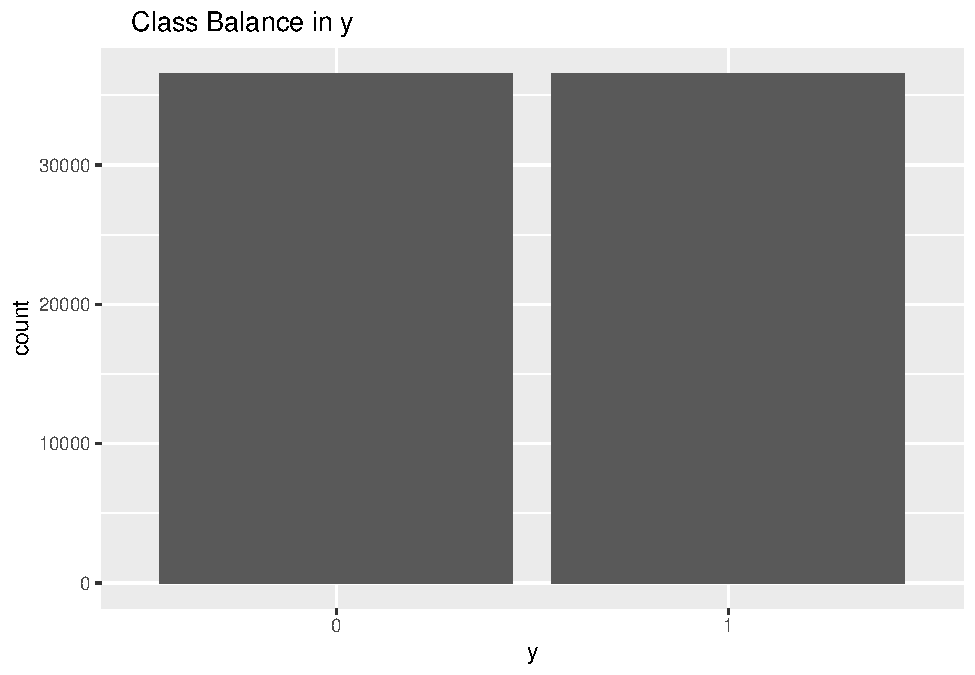
\includegraphics{part1_files/figure-latex/unnamed-chunk-12-1.pdf}

checking for NA's

\begin{Shaded}
\begin{Highlighting}[]
\FunctionTok{print}\NormalTok{(}\FunctionTok{paste}\NormalTok{(}\StringTok{"\# of NA\textquotesingle{}s"}\NormalTok{, }\FunctionTok{sum}\NormalTok{(}\FunctionTok{is.na}\NormalTok{(data))))}
\end{Highlighting}
\end{Shaded}

\begin{verbatim}
## [1] "# of NA's 0"
\end{verbatim}

checking for unknowns

\begin{Shaded}
\begin{Highlighting}[]
\FunctionTok{where\_is\_unknown}\NormalTok{(data)}
\end{Highlighting}
\end{Shaded}

\begin{verbatim}
## [1] "There are no unknown values in the dataframe"
\end{verbatim}

since there are no unknown values and no NA's, lastly checking for
increase in row count in dataframe

\begin{Shaded}
\begin{Highlighting}[]
\FunctionTok{cat}\NormalTok{(}\StringTok{"New row count is"}\NormalTok{,}\FunctionTok{nrow}\NormalTok{(data))}
\end{Highlighting}
\end{Shaded}

\begin{verbatim}
## New row count is 73096
\end{verbatim}

\hypertarget{train-test-split}{%
\paragraph{Train Test Split}\label{train-test-split}}

splitting 80/20 into train and test

\begin{Shaded}
\begin{Highlighting}[]
\FunctionTok{set.seed}\NormalTok{(}\DecValTok{3}\NormalTok{)}
\NormalTok{i }\OtherTok{\textless{}{-}} \FunctionTok{sample}\NormalTok{(}\DecValTok{1}\SpecialCharTok{:}\FunctionTok{nrow}\NormalTok{(data), }\FunctionTok{nrow}\NormalTok{(data)}\SpecialCharTok{*}\FloatTok{0.80}\NormalTok{, }\AttributeTok{replace =} \ConstantTok{FALSE}\NormalTok{)}
\NormalTok{train }\OtherTok{\textless{}{-}}\NormalTok{ data[i,]}
\NormalTok{test }\OtherTok{\textless{}{-}}\NormalTok{ data[}\SpecialCharTok{{-}}\NormalTok{i,]}
\FunctionTok{dim}\NormalTok{(train)}
\end{Highlighting}
\end{Shaded}

\begin{verbatim}
## [1] 58476    18
\end{verbatim}

\begin{Shaded}
\begin{Highlighting}[]
\FunctionTok{dim}\NormalTok{(test)}
\end{Highlighting}
\end{Shaded}

\begin{verbatim}
## [1] 14620    18
\end{verbatim}

\hypertarget{general-eda}{%
\subsubsection{General EDA}\label{general-eda}}

plotting correlation matrix

\begin{Shaded}
\begin{Highlighting}[]
\NormalTok{train}\SpecialCharTok{$}\NormalTok{y }\OtherTok{\textless{}{-}} \FunctionTok{encode}\NormalTok{(train,}\StringTok{\textquotesingle{}y\textquotesingle{}}\NormalTok{)}
\NormalTok{C }\OtherTok{\textless{}{-}} \FunctionTok{cor}\NormalTok{(train)}
\FunctionTok{corrplot}\NormalTok{(C, }\AttributeTok{method=}\StringTok{\textquotesingle{}color\textquotesingle{}}\NormalTok{, }\AttributeTok{order =} \StringTok{\textquotesingle{}alphabet\textquotesingle{}}\NormalTok{)}
\end{Highlighting}
\end{Shaded}

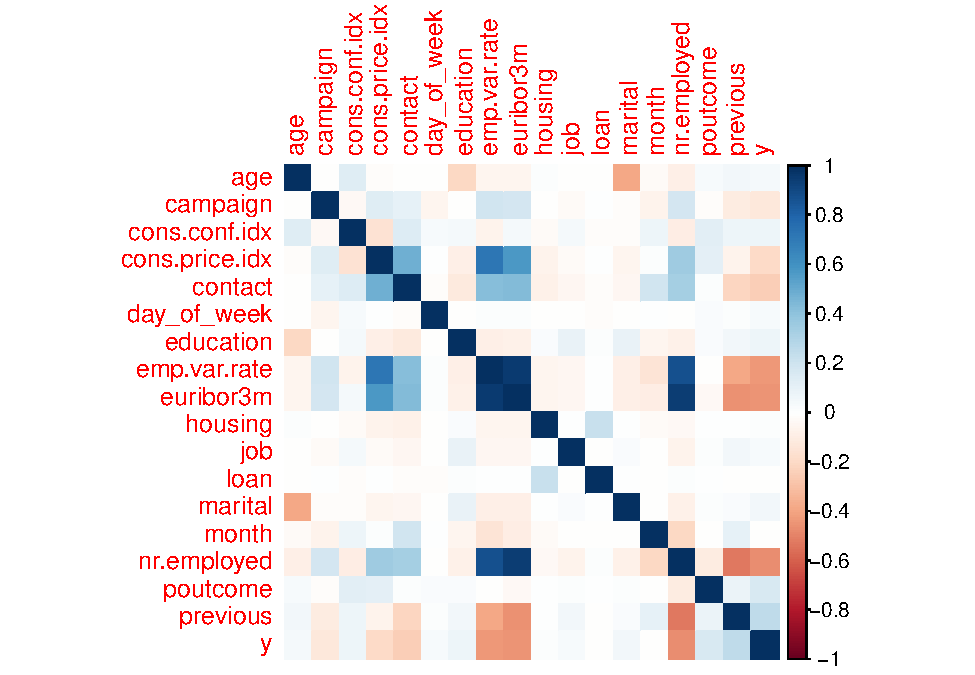
\includegraphics{part1_files/figure-latex/unnamed-chunk-17-1.pdf}

looking more specifically relative to `y'

\begin{Shaded}
\begin{Highlighting}[]
\NormalTok{C[,}\StringTok{\textquotesingle{}y\textquotesingle{}}\NormalTok{]}
\end{Highlighting}
\end{Shaded}

\begin{verbatim}
##            age            job        marital      education        housing 
##    0.036011227    0.042628178    0.056017858    0.079706893    0.017643083 
##           loan        contact          month    day_of_week       campaign 
##   -0.005310177   -0.247008029   -0.008042060    0.027354454   -0.124933072 
##       previous       poutcome   emp.var.rate cons.price.idx  cons.conf.idx 
##    0.260404696    0.160172402   -0.426317731   -0.197507679    0.077062494 
##      euribor3m    nr.employed              y 
##   -0.441863630   -0.461524510    1.000000000
\end{verbatim}

it looks like euribor3m, nr.employed, emp.var.rate have the strongest
negative correlation with y, and previous and poutcome, have the
strongest positive correlation.

\hypertarget{linear-regression}{%
\subsubsection{Linear Regression}\label{linear-regression}}

to explore more, making base model for all independents against `y'

\begin{Shaded}
\begin{Highlighting}[]
\FunctionTok{set.seed}\NormalTok{(}\DecValTok{10}\NormalTok{)}
\NormalTok{base }\OtherTok{\textless{}{-}} \FunctionTok{lm}\NormalTok{(y}\SpecialCharTok{\textasciitilde{}}\NormalTok{.,}\AttributeTok{data=}\NormalTok{train)}
\FunctionTok{summary}\NormalTok{(base)}
\end{Highlighting}
\end{Shaded}

\begin{verbatim}
## 
## Call:
## lm(formula = y ~ ., data = train)
## 
## Residuals:
##     Min      1Q  Median      3Q     Max 
## -1.1377 -0.3189 -0.1125  0.3216  0.9098 
## 
## Coefficients:
##                  Estimate Std. Error t value Pr(>|t|)    
## (Intercept)    -2.822e+00  1.518e+00  -1.859 0.063086 .  
## age            -3.072e-05  1.674e-04  -0.183 0.854417    
## job             6.325e-04  4.462e-04   1.417 0.156375    
## marital         8.096e-03  2.265e-03   3.574 0.000351 ***
## education       4.251e-03  7.702e-04   5.519 3.42e-08 ***
## housing        -3.855e-03  3.370e-03  -1.144 0.252732    
## loan            1.771e-05  4.613e-03   0.004 0.996936    
## contact        -1.434e-01  5.477e-03 -26.176  < 2e-16 ***
## month          -2.235e-02  9.131e-04 -24.477  < 2e-16 ***
## day_of_week     7.699e-03  1.283e-03   6.003 1.95e-09 ***
## campaign       -6.630e-03  7.742e-04  -8.563  < 2e-16 ***
## previous        9.467e-03  3.091e-03   3.063 0.002191 ** 
## poutcome        1.142e-01  3.936e-03  29.022  < 2e-16 ***
## emp.var.rate   -1.901e-01  6.248e-03 -30.426  < 2e-16 ***
## cons.price.idx  1.484e-01  9.427e-03  15.746  < 2e-16 ***
## cons.conf.idx   1.822e-03  5.933e-04   3.071 0.002135 ** 
## euribor3m       1.297e-01  8.863e-03  14.639  < 2e-16 ***
## nr.employed    -2.136e-03  1.502e-04 -14.219  < 2e-16 ***
## ---
## Signif. codes:  0 '***' 0.001 '**' 0.01 '*' 0.05 '.' 0.1 ' ' 1
## 
## Residual standard error: 0.4305 on 58458 degrees of freedom
## Multiple R-squared:  0.2587, Adjusted R-squared:  0.2585 
## F-statistic:  1200 on 17 and 58458 DF,  p-value: < 2.2e-16
\end{verbatim}

the insignificants appear to be age, job, housing, and loan, removing
these and redoing model

\begin{Shaded}
\begin{Highlighting}[]
\FunctionTok{set.seed}\NormalTok{(}\DecValTok{11}\NormalTok{)}
\NormalTok{m1 }\OtherTok{\textless{}{-}} \FunctionTok{lm}\NormalTok{(y}\SpecialCharTok{\textasciitilde{}}\NormalTok{.,}\AttributeTok{data=}\FunctionTok{subset}\NormalTok{(train,}\AttributeTok{select =} \SpecialCharTok{{-}}\FunctionTok{c}\NormalTok{(age,job,housing,loan)))}
\FunctionTok{summary}\NormalTok{(m1)}
\end{Highlighting}
\end{Shaded}

\begin{verbatim}
## 
## Call:
## lm(formula = y ~ ., data = subset(train, select = -c(age, job, 
##     housing, loan)))
## 
## Residuals:
##     Min      1Q  Median      3Q     Max 
## -1.1315 -0.3191 -0.1113  0.3214  0.9087 
## 
## Coefficients:
##                  Estimate Std. Error t value Pr(>|t|)    
## (Intercept)    -2.8345001  1.5149620  -1.871  0.06135 .  
## marital         0.0082916  0.0020930   3.962 7.45e-05 ***
## education       0.0043526  0.0007522   5.787 7.21e-09 ***
## contact        -0.1433145  0.0054745 -26.179  < 2e-16 ***
## month          -0.0223416  0.0009093 -24.571  < 2e-16 ***
## day_of_week     0.0076898  0.0012824   5.996 2.03e-09 ***
## campaign       -0.0066429  0.0007741  -8.581  < 2e-16 ***
## previous        0.0095377  0.0030897   3.087  0.00202 ** 
## poutcome        0.1141661  0.0039351  29.012  < 2e-16 ***
## emp.var.rate   -0.1900807  0.0062455 -30.435  < 2e-16 ***
## cons.price.idx  0.1486112  0.0094157  15.783  < 2e-16 ***
## cons.conf.idx   0.0018405  0.0005919   3.109  0.00188 ** 
## euribor3m       0.1297746  0.0088470  14.669  < 2e-16 ***
## nr.employed    -0.0021377  0.0001498 -14.271  < 2e-16 ***
## ---
## Signif. codes:  0 '***' 0.001 '**' 0.01 '*' 0.05 '.' 0.1 ' ' 1
## 
## Residual standard error: 0.4305 on 58462 degrees of freedom
## Multiple R-squared:  0.2587, Adjusted R-squared:  0.2585 
## F-statistic:  1569 on 13 and 58462 DF,  p-value: < 2.2e-16
\end{verbatim}

every predictor is significant to the regression, but still R\^{}2 is
low. let's see if scaling the independents help at all

\begin{Shaded}
\begin{Highlighting}[]
\NormalTok{minMaxScaler }\OtherTok{\textless{}{-}} \ControlFlowTok{function}\NormalTok{(v) \{}
\NormalTok{  (v}\SpecialCharTok{{-}}\FunctionTok{min}\NormalTok{(v))}\SpecialCharTok{/}\NormalTok{(}\FunctionTok{max}\NormalTok{(v)}\SpecialCharTok{{-}}\FunctionTok{min}\NormalTok{(v))}
\NormalTok{\}}
\end{Highlighting}
\end{Shaded}

\begin{Shaded}
\begin{Highlighting}[]
\NormalTok{train\_scaled }\OtherTok{\textless{}{-}} \FunctionTok{subset}\NormalTok{(train,}\AttributeTok{select =} \SpecialCharTok{{-}}\FunctionTok{c}\NormalTok{(age,job,housing,loan))}
\NormalTok{train\_scaled[,}\SpecialCharTok{{-}}\FunctionTok{ncol}\NormalTok{(train\_scaled)] }\OtherTok{\textless{}{-}} \FunctionTok{lapply}\NormalTok{(train\_scaled[, }\SpecialCharTok{{-}}\FunctionTok{ncol}\NormalTok{(train\_scaled)],minMaxScaler)}
\FunctionTok{head}\NormalTok{(train\_scaled)}
\end{Highlighting}
\end{Shaded}

\begin{verbatim}
##         marital education contact     month day_of_week   campaign  previous
## 52922 1.0000000 0.8571429       0 0.0000000        0.50 0.00000000 0.0000000
## 41352 0.0000000 1.0000000       0 0.6666667        0.25 0.00000000 0.0000000
## 36520 0.6666667 1.0000000       0 0.7777778        0.50 0.00000000 0.0000000
## 66541 1.0000000 0.5714286       0 0.4444444        0.50 0.00000000 0.0000000
## 6120  1.0000000 0.5714286       1 0.6666667        0.75 0.05454545 0.0000000
## 51849 0.6666667 1.0000000       1 0.0000000        0.50 0.00000000 0.2857143
##       poutcome emp.var.rate cons.price.idx cons.conf.idx   euribor3m
## 52922      0.5    0.3333333      0.6032736     0.6778243 0.001360236
## 41352      0.5    0.3333333      0.2696804     0.1924686 0.138290637
## 36520      0.5    0.4791667      1.0000000     0.0000000 0.092269327
## 66541      0.5    0.1041667      0.2969602     0.4184100 0.141917932
## 6120       0.5    0.9375000      0.6987529     0.6025105 0.957379279
## 51849      1.0    0.3333333      0.6032736     0.6778243 0.002267060
##       nr.employed y
## 52922   0.1705104 1
## 41352   0.5122873 1
## 36520   0.0000000 0
## 66541   0.4257089 1
## 6120    0.8597353 0
## 51849   0.1705104 1
\end{verbatim}

\begin{Shaded}
\begin{Highlighting}[]
\FunctionTok{set.seed}\NormalTok{(}\DecValTok{13}\NormalTok{)}
\NormalTok{m2 }\OtherTok{\textless{}{-}} \FunctionTok{lm}\NormalTok{(y}\SpecialCharTok{\textasciitilde{}}\NormalTok{.,}\AttributeTok{data=}\NormalTok{train\_scaled)}
\FunctionTok{summary}\NormalTok{(m2)}
\end{Highlighting}
\end{Shaded}

\begin{verbatim}
## 
## Call:
## lm(formula = y ~ ., data = train_scaled)
## 
## Residuals:
##     Min      1Q  Median      3Q     Max 
## -1.1315 -0.3191 -0.1113  0.3214  0.9087 
## 
## Coefficients:
##                 Estimate Std. Error t value Pr(>|t|)    
## (Intercept)     0.885111   0.025792  34.317  < 2e-16 ***
## marital         0.024875   0.006279   3.962 7.45e-05 ***
## education       0.030468   0.005265   5.787 7.21e-09 ***
## contact        -0.143315   0.005475 -26.179  < 2e-16 ***
## month          -0.201075   0.008183 -24.571  < 2e-16 ***
## day_of_week     0.030759   0.005130   5.996 2.03e-09 ***
## campaign       -0.365360   0.042577  -8.581  < 2e-16 ***
## previous        0.066764   0.021628   3.087  0.00202 ** 
## poutcome        0.228332   0.007870  29.012  < 2e-16 ***
## emp.var.rate   -0.912388   0.029979 -30.435  < 2e-16 ***
## cons.price.idx  0.381336   0.024161  15.783  < 2e-16 ***
## cons.conf.idx   0.043988   0.014148   3.109  0.00188 ** 
## euribor3m       0.572436   0.039024  14.669  < 2e-16 ***
## nr.employed    -0.565433   0.039620 -14.271  < 2e-16 ***
## ---
## Signif. codes:  0 '***' 0.001 '**' 0.01 '*' 0.05 '.' 0.1 ' ' 1
## 
## Residual standard error: 0.4305 on 58462 degrees of freedom
## Multiple R-squared:  0.2587, Adjusted R-squared:  0.2585 
## F-statistic:  1569 on 13 and 58462 DF,  p-value: < 2.2e-16
\end{verbatim}

\begin{Shaded}
\begin{Highlighting}[]
\FunctionTok{par}\NormalTok{(}\AttributeTok{mfrow=}\FunctionTok{c}\NormalTok{(}\DecValTok{2}\NormalTok{,}\DecValTok{2}\NormalTok{))}
\FunctionTok{plot}\NormalTok{(m2)}
\end{Highlighting}
\end{Shaded}

\includegraphics{part1_files/figure-latex/unnamed-chunk-24-1.pdf}

\begin{Shaded}
\begin{Highlighting}[]
\FunctionTok{par}\NormalTok{(}\AttributeTok{mfrow=}\FunctionTok{c}\NormalTok{(}\DecValTok{1}\NormalTok{,}\DecValTok{1}\NormalTok{))}
\end{Highlighting}
\end{Shaded}

true to form, scaling does not impact the regression results. Both
R\^{}2 and the adjusted R\^{}2 are staying low. we will use the model
`m1' for prediction as `m2' doesn't appear to be doing much better.

\hypertarget{linear-regression-evaluation}{%
\paragraph{Linear Regression
Evaluation}\label{linear-regression-evaluation}}

create model for `m1' once again (no scaling)

\begin{Shaded}
\begin{Highlighting}[]
\FunctionTok{set.seed}\NormalTok{(}\DecValTok{11}\NormalTok{)}
\NormalTok{m1 }\OtherTok{\textless{}{-}} \FunctionTok{lm}\NormalTok{(y}\SpecialCharTok{\textasciitilde{}}\NormalTok{.,}\AttributeTok{data=}\FunctionTok{subset}\NormalTok{(train,}\AttributeTok{select =} \SpecialCharTok{{-}}\FunctionTok{c}\NormalTok{(age,job,housing,loan)))}
\FunctionTok{summary}\NormalTok{(m1)}
\end{Highlighting}
\end{Shaded}

\begin{verbatim}
## 
## Call:
## lm(formula = y ~ ., data = subset(train, select = -c(age, job, 
##     housing, loan)))
## 
## Residuals:
##     Min      1Q  Median      3Q     Max 
## -1.1315 -0.3191 -0.1113  0.3214  0.9087 
## 
## Coefficients:
##                  Estimate Std. Error t value Pr(>|t|)    
## (Intercept)    -2.8345001  1.5149620  -1.871  0.06135 .  
## marital         0.0082916  0.0020930   3.962 7.45e-05 ***
## education       0.0043526  0.0007522   5.787 7.21e-09 ***
## contact        -0.1433145  0.0054745 -26.179  < 2e-16 ***
## month          -0.0223416  0.0009093 -24.571  < 2e-16 ***
## day_of_week     0.0076898  0.0012824   5.996 2.03e-09 ***
## campaign       -0.0066429  0.0007741  -8.581  < 2e-16 ***
## previous        0.0095377  0.0030897   3.087  0.00202 ** 
## poutcome        0.1141661  0.0039351  29.012  < 2e-16 ***
## emp.var.rate   -0.1900807  0.0062455 -30.435  < 2e-16 ***
## cons.price.idx  0.1486112  0.0094157  15.783  < 2e-16 ***
## cons.conf.idx   0.0018405  0.0005919   3.109  0.00188 ** 
## euribor3m       0.1297746  0.0088470  14.669  < 2e-16 ***
## nr.employed    -0.0021377  0.0001498 -14.271  < 2e-16 ***
## ---
## Signif. codes:  0 '***' 0.001 '**' 0.01 '*' 0.05 '.' 0.1 ' ' 1
## 
## Residual standard error: 0.4305 on 58462 degrees of freedom
## Multiple R-squared:  0.2587, Adjusted R-squared:  0.2585 
## F-statistic:  1569 on 13 and 58462 DF,  p-value: < 2.2e-16
\end{verbatim}

get predictions and measure accuracy

\begin{Shaded}
\begin{Highlighting}[]
\FunctionTok{set.seed}\NormalTok{(}\DecValTok{21}\NormalTok{)}
\NormalTok{probas }\OtherTok{\textless{}{-}} \FunctionTok{predict}\NormalTok{(m1, }\AttributeTok{newdata =}\NormalTok{ test, }\AttributeTok{type=}\StringTok{"response"}\NormalTok{)}
\NormalTok{pred }\OtherTok{\textless{}{-}} \FunctionTok{ifelse}\NormalTok{(probas}\SpecialCharTok{\textgreater{}}\FloatTok{0.5}\NormalTok{, }\DecValTok{1}\NormalTok{, }\DecValTok{0}\NormalTok{)}
\NormalTok{acc }\OtherTok{\textless{}{-}} \FunctionTok{mean}\NormalTok{(pred}\SpecialCharTok{==}\NormalTok{test}\SpecialCharTok{$}\NormalTok{y)}
\FunctionTok{print}\NormalTok{(}\FunctionTok{paste}\NormalTok{(}\StringTok{"Accuracy = "}\NormalTok{, }\FunctionTok{round}\NormalTok{(acc,}\DecValTok{3}\NormalTok{)))}
\end{Highlighting}
\end{Shaded}

\begin{verbatim}
## [1] "Accuracy =  0.735"
\end{verbatim}

\begin{Shaded}
\begin{Highlighting}[]
\FunctionTok{print}\NormalTok{(}\FunctionTok{paste}\NormalTok{(}\StringTok{"Correlation = "}\NormalTok{,}\FunctionTok{round}\NormalTok{(}\FunctionTok{cor}\NormalTok{(probas,}\FunctionTok{as.numeric}\NormalTok{(test}\SpecialCharTok{$}\NormalTok{y)}\SpecialCharTok{{-}}\DecValTok{1}\NormalTok{),}\DecValTok{3}\NormalTok{)))}
\end{Highlighting}
\end{Shaded}

\begin{verbatim}
## [1] "Correlation =  0.518"
\end{verbatim}

construct confusion matrix for easy visualization

\begin{Shaded}
\begin{Highlighting}[]
\FunctionTok{confusionMatrix}\NormalTok{(}\FunctionTok{as.factor}\NormalTok{(pred), }\AttributeTok{reference=}\NormalTok{test}\SpecialCharTok{$}\NormalTok{y)}
\end{Highlighting}
\end{Shaded}

\begin{verbatim}
## Confusion Matrix and Statistics
## 
##           Reference
## Prediction    0    1
##          0 5907 2417
##          1 1459 4837
##                                          
##                Accuracy : 0.7349         
##                  95% CI : (0.7276, 0.742)
##     No Information Rate : 0.5038         
##     P-Value [Acc > NIR] : < 2.2e-16      
##                                          
##                   Kappa : 0.4692         
##                                          
##  Mcnemar's Test P-Value : < 2.2e-16      
##                                          
##             Sensitivity : 0.8019         
##             Specificity : 0.6668         
##          Pos Pred Value : 0.7096         
##          Neg Pred Value : 0.7683         
##              Prevalence : 0.5038         
##          Detection Rate : 0.4040         
##    Detection Prevalence : 0.5694         
##       Balanced Accuracy : 0.7344         
##                                          
##        'Positive' Class : 0              
## 
\end{verbatim}

construct ROC plot \& show auc

\begin{Shaded}
\begin{Highlighting}[]
\FunctionTok{set.seed}\NormalTok{(}\DecValTok{31}\NormalTok{)}
\NormalTok{pred }\OtherTok{\textless{}{-}} \FunctionTok{prediction}\NormalTok{(probas,test}\SpecialCharTok{$}\NormalTok{y)}
\NormalTok{roc }\OtherTok{\textless{}{-}} \FunctionTok{performance}\NormalTok{(pred, }\AttributeTok{measure=}\StringTok{"tpr"}\NormalTok{, }\AttributeTok{x.measure=}\StringTok{"fpr"}\NormalTok{)}
\FunctionTok{plot}\NormalTok{(roc)}
\end{Highlighting}
\end{Shaded}

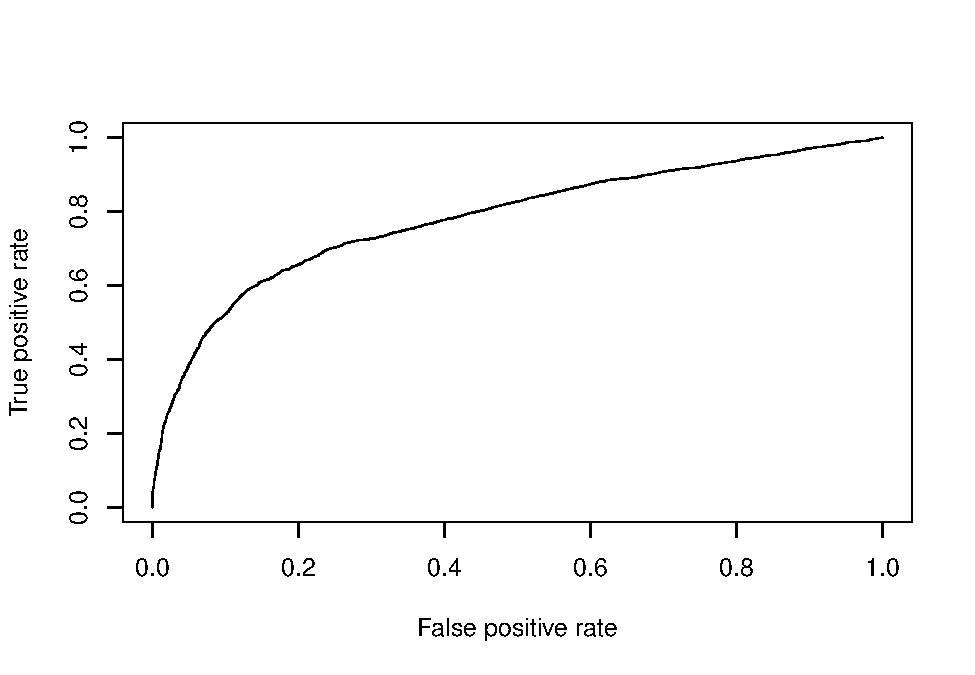
\includegraphics{part1_files/figure-latex/unnamed-chunk-28-1.pdf}

\begin{Shaded}
\begin{Highlighting}[]
\FunctionTok{cat}\NormalTok{(}\StringTok{"auc ="}\NormalTok{, }\FunctionTok{round}\NormalTok{(}\FunctionTok{performance}\NormalTok{(pred,}\AttributeTok{measure=}\StringTok{"auc"}\NormalTok{)}\SpecialCharTok{@}\NormalTok{y.values[[}\DecValTok{1}\NormalTok{]],}\DecValTok{3}\NormalTok{))}
\end{Highlighting}
\end{Shaded}

\begin{verbatim}
## auc = 0.789
\end{verbatim}

Overall, the linear regression model was predicting at around 73\%
accuracy. The correlation is around 51\%. The model seemed to be able to
distinguish between positive and negative classes for the `y' feature
though, with auc of about 78\%.

Let's see if KNN regression can do more justice.

\hypertarget{knn-regression}{%
\subsubsection{KNN Regression}\label{knn-regression}}

For KNN we will use the scaled version of the training sample. We will
need to scale everything in test as well except for the the target `y'

\begin{Shaded}
\begin{Highlighting}[]
\NormalTok{test\_scaled }\OtherTok{\textless{}{-}} \FunctionTok{subset}\NormalTok{(test,}\AttributeTok{select =} \SpecialCharTok{{-}}\FunctionTok{c}\NormalTok{(age,job,housing,loan))}
\NormalTok{test\_scaled[,}\SpecialCharTok{{-}}\FunctionTok{ncol}\NormalTok{(test\_scaled)] }\OtherTok{\textless{}{-}} \FunctionTok{lapply}\NormalTok{(test\_scaled[, }\SpecialCharTok{{-}}\FunctionTok{ncol}\NormalTok{(test\_scaled)],minMaxScaler)}
\end{Highlighting}
\end{Shaded}

Fit the scaled training data to the model

\begin{Shaded}
\begin{Highlighting}[]
\NormalTok{kr1 }\OtherTok{\textless{}{-}} \FunctionTok{knnreg}\NormalTok{(train\_scaled[,}\SpecialCharTok{{-}}\FunctionTok{ncol}\NormalTok{(train\_scaled)], train\_scaled[,}\StringTok{\textquotesingle{}y\textquotesingle{}}\NormalTok{])}
\FunctionTok{summary}\NormalTok{(kr1)}
\end{Highlighting}
\end{Shaded}

\begin{verbatim}
##         Length Class  Mode   
## learn   2      -none- list   
## k       1      -none- numeric
## theDots 0      -none- list
\end{verbatim}

\begin{Shaded}
\begin{Highlighting}[]
\NormalTok{probas }\OtherTok{\textless{}{-}} \FunctionTok{predict}\NormalTok{(kr1, }\AttributeTok{newdata =}\NormalTok{ test\_scaled[,}\SpecialCharTok{{-}}\FunctionTok{ncol}\NormalTok{(test\_scaled)], }\AttributeTok{type=}\StringTok{"response"}\NormalTok{)}
\NormalTok{pred }\OtherTok{\textless{}{-}} \FunctionTok{ifelse}\NormalTok{(probas}\SpecialCharTok{\textgreater{}}\FloatTok{0.5}\NormalTok{, }\DecValTok{1}\NormalTok{, }\DecValTok{0}\NormalTok{)}
\NormalTok{cor\_kr1 }\OtherTok{\textless{}{-}} \FunctionTok{cor}\NormalTok{(pred,}\FunctionTok{as.numeric}\NormalTok{(test}\SpecialCharTok{$}\NormalTok{y)}\SpecialCharTok{{-}}\DecValTok{1}\NormalTok{)}
\FunctionTok{cat}\NormalTok{(}\StringTok{"correlation="}\NormalTok{, }\FunctionTok{round}\NormalTok{(cor\_kr1,}\DecValTok{3}\NormalTok{))}
\end{Highlighting}
\end{Shaded}

\begin{verbatim}
## correlation= 0.575
\end{verbatim}

construct confusion matrix for easy visualization

\begin{Shaded}
\begin{Highlighting}[]
\FunctionTok{confusionMatrix}\NormalTok{(}\FunctionTok{as.factor}\NormalTok{(pred), }\AttributeTok{reference=}\NormalTok{test}\SpecialCharTok{$}\NormalTok{y)}
\end{Highlighting}
\end{Shaded}

\begin{verbatim}
## Confusion Matrix and Statistics
## 
##           Reference
## Prediction    0    1
##          0 5293 1075
##          1 2073 6179
##                                           
##                Accuracy : 0.7847          
##                  95% CI : (0.7779, 0.7913)
##     No Information Rate : 0.5038          
##     P-Value [Acc > NIR] : < 2.2e-16       
##                                           
##                   Kappa : 0.5698          
##                                           
##  Mcnemar's Test P-Value : < 2.2e-16       
##                                           
##             Sensitivity : 0.7186          
##             Specificity : 0.8518          
##          Pos Pred Value : 0.8312          
##          Neg Pred Value : 0.7488          
##              Prevalence : 0.5038          
##          Detection Rate : 0.3620          
##    Detection Prevalence : 0.4356          
##       Balanced Accuracy : 0.7852          
##                                           
##        'Positive' Class : 0               
## 
\end{verbatim}

Correlation went up, let's see if we can select the best k to maximize
it \& minimize mse

\begin{Shaded}
\begin{Highlighting}[]
\NormalTok{cor\_kr }\OtherTok{\textless{}{-}} \FunctionTok{rep}\NormalTok{(}\DecValTok{0}\NormalTok{,}\DecValTok{20}\NormalTok{)}
\NormalTok{mse\_kr }\OtherTok{\textless{}{-}} \FunctionTok{rep}\NormalTok{(}\DecValTok{0}\NormalTok{,}\DecValTok{20}\NormalTok{)}
\NormalTok{test\_y\_num }\OtherTok{\textless{}{-}} \FunctionTok{encode}\NormalTok{(test,}\StringTok{\textquotesingle{}y\textquotesingle{}}\NormalTok{)}
\NormalTok{i }\OtherTok{\textless{}{-}} \DecValTok{1}
\ControlFlowTok{for}\NormalTok{(k }\ControlFlowTok{in} \FunctionTok{seq}\NormalTok{(}\DecValTok{1}\NormalTok{,}\DecValTok{39}\NormalTok{,}\DecValTok{2}\NormalTok{)) \{}
\NormalTok{  fit\_k }\OtherTok{\textless{}{-}} \FunctionTok{knnreg}\NormalTok{(train\_scaled[,}\SpecialCharTok{{-}}\FunctionTok{ncol}\NormalTok{(train\_scaled)], train\_scaled}\SpecialCharTok{$}\NormalTok{y, }\AttributeTok{k=}\NormalTok{k)}
\NormalTok{  pred\_k }\OtherTok{\textless{}{-}} \FunctionTok{predict}\NormalTok{(fit\_k, test\_scaled[,}\SpecialCharTok{{-}}\FunctionTok{ncol}\NormalTok{(test\_scaled)])}
\NormalTok{  cor\_kr[i] }\OtherTok{\textless{}{-}} \FunctionTok{cor}\NormalTok{(pred\_k,test\_y\_num)}
\NormalTok{  mse\_kr[i] }\OtherTok{\textless{}{-}} \FunctionTok{mean}\NormalTok{((pred\_k }\SpecialCharTok{{-}}\NormalTok{ test\_y\_num)}\SpecialCharTok{\^{}}\DecValTok{2}\NormalTok{)}
  \FunctionTok{print}\NormalTok{(}\FunctionTok{paste}\NormalTok{(}\StringTok{"k="}\NormalTok{,k,cor\_kr[i],mse\_kr[i]))}
\NormalTok{  i }\OtherTok{\textless{}{-}}\NormalTok{ i}\SpecialCharTok{+}\DecValTok{1}
\NormalTok{\}}
\end{Highlighting}
\end{Shaded}

\begin{verbatim}
## [1] "k= 1 0.678584031290735 0.143430605846082"
## [1] "k= 3 0.675226022855891 0.142994992230485"
## [1] "k= 5 0.664323400097104 0.145956738247432"
## [1] "k= 7 0.647627466543953 0.15051513040124"
## [1] "k= 9 0.636746103053741 0.153073334010753"
## [1] "k= 11 0.626572165089006 0.155538009337429"
## [1] "k= 13 0.619949797574762 0.157033786195962"
## [1] "k= 15 0.613863315639075 0.15847531228401"
## [1] "k= 17 0.605539312026449 0.160694286944949"
## [1] "k= 19 0.604529266776346 0.160629392559089"
## [1] "k= 21 0.599090741210623 0.162098699129918"
## [1] "k= 23 0.597038256087805 0.162475497757066"
## [1] "k= 25 0.592975222843602 0.163577268934292"
## [1] "k= 27 0.591416488115984 0.163852794787533"
## [1] "k= 29 0.588172168314349 0.164678101953342"
## [1] "k= 31 0.586828210063501 0.164949253668353"
## [1] "k= 33 0.583970653353727 0.165710517256386"
## [1] "k= 35 0.580416253865704 0.166703412516878"
## [1] "k= 37 0.579728994450879 0.166833933289052"
## [1] "k= 39 0.578853136144378 0.167021550467218"
\end{verbatim}

\hypertarget{knn-regression-evaluation}{%
\subsection{KNN Regression Evaluation}\label{knn-regression-evaluation}}

coincidentally, the correlation is in sorted order, k=1 produces the
highest. However, the lowest mse is when k=3. Since the loss in
correlation from k=1 to k=3 is not too drastic, we will use k=3 to
train.

\begin{Shaded}
\begin{Highlighting}[]
\NormalTok{fit\_3 }\OtherTok{\textless{}{-}} \FunctionTok{knnreg}\NormalTok{(train\_scaled[,}\SpecialCharTok{{-}}\FunctionTok{ncol}\NormalTok{(train\_scaled)], train\_scaled}\SpecialCharTok{$}\NormalTok{y, }\AttributeTok{k=}\DecValTok{3}\NormalTok{)}
\FunctionTok{summary}\NormalTok{(fit\_3)}
\end{Highlighting}
\end{Shaded}

\begin{verbatim}
##         Length Class  Mode   
## learn   2      -none- list   
## k       1      -none- numeric
## theDots 0      -none- list
\end{verbatim}

\begin{Shaded}
\begin{Highlighting}[]
\NormalTok{predictions\_3 }\OtherTok{\textless{}{-}} \FunctionTok{predict}\NormalTok{(fit\_3, test\_scaled[,}\SpecialCharTok{{-}}\FunctionTok{ncol}\NormalTok{(test\_scaled)])}
\NormalTok{cor\_kr3 }\OtherTok{\textless{}{-}} \FunctionTok{cor}\NormalTok{(predictions\_3, test\_y\_num)}
\NormalTok{mse\_kr3 }\OtherTok{\textless{}{-}} \FunctionTok{mean}\NormalTok{((predictions\_3 }\SpecialCharTok{{-}}\NormalTok{ test\_y\_num)}\SpecialCharTok{\^{}}\DecValTok{2}\NormalTok{)}
\FunctionTok{print}\NormalTok{(}\FunctionTok{paste}\NormalTok{(}\StringTok{"corr="}\NormalTok{, cor\_kr3))}
\end{Highlighting}
\end{Shaded}

\begin{verbatim}
## [1] "corr= 0.675226022855891"
\end{verbatim}

\begin{Shaded}
\begin{Highlighting}[]
\FunctionTok{print}\NormalTok{(}\FunctionTok{paste}\NormalTok{(}\StringTok{"mse="}\NormalTok{, mse\_kr3))}
\end{Highlighting}
\end{Shaded}

\begin{verbatim}
## [1] "mse= 0.142994992230485"
\end{verbatim}

\begin{Shaded}
\begin{Highlighting}[]
\FunctionTok{set.seed}\NormalTok{(}\DecValTok{101}\NormalTok{)}
\NormalTok{km2 }\OtherTok{\textless{}{-}} \FunctionTok{knnreg}\NormalTok{(y}\SpecialCharTok{\textasciitilde{}}\NormalTok{., }\AttributeTok{data=}\NormalTok{train\_scaled, }\AttributeTok{k=}\DecValTok{3}\NormalTok{)}
\NormalTok{probas }\OtherTok{\textless{}{-}} \FunctionTok{predict}\NormalTok{(km2, }\AttributeTok{newdata =}\NormalTok{ test\_scaled[,}\SpecialCharTok{{-}}\FunctionTok{ncol}\NormalTok{(test\_scaled)], }\AttributeTok{type=}\StringTok{"response"}\NormalTok{)}
\NormalTok{pred }\OtherTok{\textless{}{-}} \FunctionTok{ifelse}\NormalTok{(probas}\SpecialCharTok{\textgreater{}}\FloatTok{0.5}\NormalTok{, }\DecValTok{1}\NormalTok{, }\DecValTok{0}\NormalTok{)}
\FunctionTok{confusionMatrix}\NormalTok{(}\FunctionTok{as.factor}\NormalTok{(pred), }\AttributeTok{reference=}\NormalTok{test}\SpecialCharTok{$}\NormalTok{y)}
\end{Highlighting}
\end{Shaded}

\begin{verbatim}
## Confusion Matrix and Statistics
## 
##           Reference
## Prediction    0    1
##          0 5556 1101
##          1 1810 6153
##                                           
##                Accuracy : 0.8009          
##                  95% CI : (0.7943, 0.8073)
##     No Information Rate : 0.5038          
##     P-Value [Acc > NIR] : < 2.2e-16       
##                                           
##                   Kappa : 0.6021          
##                                           
##  Mcnemar's Test P-Value : < 2.2e-16       
##                                           
##             Sensitivity : 0.7543          
##             Specificity : 0.8482          
##          Pos Pred Value : 0.8346          
##          Neg Pred Value : 0.7727          
##              Prevalence : 0.5038          
##          Detection Rate : 0.3800          
##    Detection Prevalence : 0.4553          
##       Balanced Accuracy : 0.8012          
##                                           
##        'Positive' Class : 0               
## 
\end{verbatim}

Using the k=3, there is a slight increase in the accuracy of our model.
The sensitivity is lower than the specificity. Pointing at the model
being about 8\% better at predicting `yes' (1) responses for the target
y than `no' (0) response for the target y. Which is pretty good
considering that originally, it was that there were much more `no'
responses than `yes', resulting in imbalance. The model is predicting at
a decent rate and making fair guesses for each class of the target.

\begin{Shaded}
\begin{Highlighting}[]
\FunctionTok{set.seed}\NormalTok{(}\DecValTok{102}\NormalTok{)}
\NormalTok{pred }\OtherTok{\textless{}{-}} \FunctionTok{prediction}\NormalTok{(probas,test\_scaled}\SpecialCharTok{$}\NormalTok{y)}
\NormalTok{roc }\OtherTok{\textless{}{-}} \FunctionTok{performance}\NormalTok{(pred, }\AttributeTok{measure=}\StringTok{"tpr"}\NormalTok{, }\AttributeTok{x.measure=}\StringTok{"fpr"}\NormalTok{)}
\FunctionTok{plot}\NormalTok{(roc)}
\end{Highlighting}
\end{Shaded}

\includegraphics{part1_files/figure-latex/unnamed-chunk-37-1.pdf}

\begin{Shaded}
\begin{Highlighting}[]
\FunctionTok{cat}\NormalTok{(}\StringTok{"auc ="}\NormalTok{, }\FunctionTok{round}\NormalTok{(}\FunctionTok{performance}\NormalTok{(pred,}\AttributeTok{measure=}\StringTok{"auc"}\NormalTok{)}\SpecialCharTok{@}\NormalTok{y.values[[}\DecValTok{1}\NormalTok{]],}\DecValTok{3}\NormalTok{))}
\end{Highlighting}
\end{Shaded}

\begin{verbatim}
## auc = 0.881
\end{verbatim}

AUC ROC also increased with the change in the k value for knn. It jumped
by nearly 10\% after using the scaled features from the base model of
knnregression as well as that for the best linear regression model we
came up with.

\hypertarget{decision-tree-regression}{%
\subsubsection{Decision Tree
Regression}\label{decision-tree-regression}}

\begin{Shaded}
\begin{Highlighting}[]
\NormalTok{fit\_4 }\OtherTok{\textless{}{-}} \FunctionTok{rpart}\NormalTok{(y}\SpecialCharTok{\textasciitilde{}}\NormalTok{.,}
               \AttributeTok{data=}\NormalTok{train)}
\end{Highlighting}
\end{Shaded}

\begin{Shaded}
\begin{Highlighting}[]
\FunctionTok{summary}\NormalTok{(fit\_4)}
\end{Highlighting}
\end{Shaded}

\begin{verbatim}
## Call:
## rpart(formula = y ~ ., data = train)
##   n= 58476 
## 
##           CP nsplit rel error    xerror         xstd
## 1 0.19827105      0 1.0000000 1.0000258 1.854413e-05
## 2 0.03874644      1 0.8017289 0.8017701 2.964741e-03
## 3 0.01101605      2 0.7629825 0.7630541 3.278846e-03
## 4 0.01000000      3 0.7519665 0.7539435 3.300954e-03
## 
## Variable importance
##    nr.employed      euribor3m  cons.conf.idx   emp.var.rate cons.price.idx 
##             24             21             18             13             12 
##       poutcome          month        contact 
##              7              4              1 
## 
## Node number 1: 58476 observations,    complexity param=0.1982711
##   mean=0.5009577, MSE=0.2499991 
##   left son=2 (42400 obs) right son=3 (16076 obs)
##   Primary splits:
##       nr.employed   < 5087.65 to the right, improve=0.19827110, (0 missing)
##       euribor3m     < 3.191   to the right, improve=0.18292050, (0 missing)
##       emp.var.rate  < -0.15   to the right, improve=0.18271420, (0 missing)
##       poutcome      < 1.5     to the left,  improve=0.08895695, (0 missing)
##       cons.conf.idx < -35.45  to the left,  improve=0.08278788, (0 missing)
##   Surrogate splits:
##       euribor3m      < 1.2395  to the right, agree=0.968, adj=0.882, (0 split)
##       emp.var.rate   < -2.35   to the right, agree=0.872, adj=0.533, (0 split)
##       cons.conf.idx  < -35.45  to the left,  agree=0.867, adj=0.516, (0 split)
##       cons.price.idx < 92.7345 to the right, agree=0.837, adj=0.409, (0 split)
##       poutcome       < 1.5     to the left,  agree=0.806, adj=0.294, (0 split)
## 
## Node number 2: 42400 observations,    complexity param=0.03874644
##   mean=0.3638679, MSE=0.2314681 
##   left son=4 (37155 obs) right son=5 (5245 obs)
##   Primary splits:
##       cons.conf.idx  < -46.65  to the right, improve=0.05771530, (0 missing)
##       euribor3m      < 3.191   to the right, improve=0.05477858, (0 missing)
##       emp.var.rate   < -0.15   to the right, improve=0.05463425, (0 missing)
##       nr.employed    < 5183.65 to the right, improve=0.05463425, (0 missing)
##       cons.price.idx < 93.1375 to the right, improve=0.05463425, (0 missing)
##   Surrogate splits:
##       month          < 0.5     to the right, agree=0.979, adj=0.827, (0 split)
##       cons.price.idx < 92.868  to the right, agree=0.897, adj=0.169, (0 split)
##       age            < 60.5    to the left,  agree=0.885, adj=0.068, (0 split)
##       previous       < 2.5     to the left,  agree=0.876, adj=0.000, (0 split)
## 
## Node number 3: 16076 observations
##   mean=0.862528, MSE=0.1185735 
## 
## Node number 4: 37155 observations,    complexity param=0.01101605
##   mean=0.3204414, MSE=0.2177587 
##   left son=8 (12083 obs) right son=9 (25072 obs)
##   Primary splits:
##       cons.price.idx < 93.956  to the right, improve=0.01990440, (0 missing)
##       contact        < 0.5     to the right, improve=0.01709743, (0 missing)
##       euribor3m      < 3.191   to the right, improve=0.01682602, (0 missing)
##       cons.conf.idx  < -44.3   to the right, improve=0.01673103, (0 missing)
##       nr.employed    < 5183.65 to the right, improve=0.01673103, (0 missing)
##   Surrogate splits:
##       contact       < 0.5     to the right, agree=0.938, adj=0.809, (0 split)
##       cons.conf.idx < -41.9   to the right, agree=0.840, adj=0.509, (0 split)
##       month         < 3.5     to the right, agree=0.684, adj=0.027, (0 split)
##       nr.employed   < 5193.4  to the left,  agree=0.677, adj=0.006, (0 split)
##       campaign      < 20.5    to the right, agree=0.675, adj=0.001, (0 split)
## 
## Node number 5: 5245 observations
##   mean=0.6714967, MSE=0.2205889 
## 
## Node number 8: 12083 observations
##   mean=0.2256062, MSE=0.1747081 
## 
## Node number 9: 25072 observations
##   mean=0.3661455, MSE=0.232083
\end{verbatim}

\begin{Shaded}
\begin{Highlighting}[]
\NormalTok{predictions\_4 }\OtherTok{\textless{}{-}} \FunctionTok{predict}\NormalTok{(fit\_4, test[,}\SpecialCharTok{{-}}\FunctionTok{ncol}\NormalTok{(test)])}
\NormalTok{cor\_kr3 }\OtherTok{\textless{}{-}} \FunctionTok{cor}\NormalTok{(predictions\_4, test\_y\_num)}
\NormalTok{mse\_kr3 }\OtherTok{\textless{}{-}} \FunctionTok{mean}\NormalTok{((predictions\_4 }\SpecialCharTok{{-}}\NormalTok{ test\_y\_num)}\SpecialCharTok{\^{}}\DecValTok{2}\NormalTok{)}
\FunctionTok{print}\NormalTok{(}\FunctionTok{paste}\NormalTok{(}\StringTok{"corr="}\NormalTok{, cor\_kr3))}
\end{Highlighting}
\end{Shaded}

\begin{verbatim}
## [1] "corr= 0.509679939497704"
\end{verbatim}

\begin{Shaded}
\begin{Highlighting}[]
\FunctionTok{print}\NormalTok{(}\FunctionTok{paste}\NormalTok{(}\StringTok{"mse="}\NormalTok{, mse\_kr3))}
\end{Highlighting}
\end{Shaded}

\begin{verbatim}
## [1] "mse= 0.185118734312541"
\end{verbatim}

\begin{Shaded}
\begin{Highlighting}[]
\NormalTok{pred }\OtherTok{\textless{}{-}} \FunctionTok{ifelse}\NormalTok{(predictions\_4}\SpecialCharTok{\textgreater{}}\FloatTok{0.5}\NormalTok{, }\DecValTok{1}\NormalTok{, }\DecValTok{0}\NormalTok{)}
\FunctionTok{confusionMatrix}\NormalTok{(}\FunctionTok{as.factor}\NormalTok{(pred), }\AttributeTok{reference=}\NormalTok{test}\SpecialCharTok{$}\NormalTok{y)}
\end{Highlighting}
\end{Shaded}

\begin{verbatim}
## Confusion Matrix and Statistics
## 
##           Reference
## Prediction    0    1
##          0 6372 2859
##          1  994 4395
##                                           
##                Accuracy : 0.7365          
##                  95% CI : (0.7292, 0.7436)
##     No Information Rate : 0.5038          
##     P-Value [Acc > NIR] : < 2.2e-16       
##                                           
##                   Kappa : 0.4719          
##                                           
##  Mcnemar's Test P-Value : < 2.2e-16       
##                                           
##             Sensitivity : 0.8651          
##             Specificity : 0.6059          
##          Pos Pred Value : 0.6903          
##          Neg Pred Value : 0.8156          
##              Prevalence : 0.5038          
##          Detection Rate : 0.4358          
##    Detection Prevalence : 0.6314          
##       Balanced Accuracy : 0.7355          
##                                           
##        'Positive' Class : 0               
## 
\end{verbatim}

\begin{Shaded}
\begin{Highlighting}[]
\FunctionTok{set.seed}\NormalTok{(}\DecValTok{404}\NormalTok{)}
\NormalTok{pred }\OtherTok{\textless{}{-}} \FunctionTok{prediction}\NormalTok{(predictions\_4,test}\SpecialCharTok{$}\NormalTok{y)}
\NormalTok{roc }\OtherTok{\textless{}{-}} \FunctionTok{performance}\NormalTok{(pred, }\AttributeTok{measure=}\StringTok{"tpr"}\NormalTok{, }\AttributeTok{x.measure=}\StringTok{"fpr"}\NormalTok{)}
\FunctionTok{plot}\NormalTok{(roc)}
\end{Highlighting}
\end{Shaded}

\includegraphics{part1_files/figure-latex/unnamed-chunk-42-1.pdf}

\begin{Shaded}
\begin{Highlighting}[]
\FunctionTok{cat}\NormalTok{(}\StringTok{"auc ="}\NormalTok{, }\FunctionTok{round}\NormalTok{(}\FunctionTok{performance}\NormalTok{(pred,}\AttributeTok{measure=}\StringTok{"auc"}\NormalTok{)}\SpecialCharTok{@}\NormalTok{y.values[[}\DecValTok{1}\NormalTok{]],}\DecValTok{3}\NormalTok{))}
\end{Highlighting}
\end{Shaded}

\begin{verbatim}
## auc = 0.77
\end{verbatim}

\end{document}
